% Les caracteristiques du document sont definies dans definition.tex
%-----------------------------------------------------------
\documentclass[a4paper,final,authoryeartwoside,11pt]{elsarticle}
\usepackage[applemac]{inputenc}
%\usepackage[dvips]{graphicx}
\usepackage{palatino,mathpazo,amssymb,amsmath,booktabs,fancybox,upgreek}
\usepackage{amsthm}
\usepackage{mathrsfs}
%-----------------------------------------------------------


%-----------------------------------------------------------
% Marges (mais o� est Omer ???)
\hoffset        = -5.4mm        
\voffset       = -7.4mm
\oddsidemargin  =   .5cm        
\evensidemargin=   .5cm
\topmargin    = 0cm
\textwidth      = 16cm  
\textheight    = 23cm
%-----------------------------------------------------------


%-----------------------------------------------------------
% Longueurs 
\renewcommand{\baselinestretch}{1.1}
\setlength{\parskip   }{3mm}
\setlength{\parindent }{5mm}
\setlength{\fboxsep   }{2mm}
\setlength{\shadowsize}{.5mm}
\cornersize*{5mm}
\numberwithin{equation}{section}
%\renewcommand{\theequation}{\thesection.\arabic{equation}}
%-----------------------------------------------------------


%-----------------------------------------------------------
% "Defs math"
\newcommand{\ddt}[1]{\frac{\partial #1}{\partial t}}
\newcommand{\ddx}[1]{\frac{\partial #1}{\partial x}}
\newcommand{\dddt}[1]{\frac{\partial^2 #1}{\partial t^2}}
\newcommand{\ddddt}[1]{\frac{\partial^3 #1}{\partial t^3}}
\newcommand{\dddddt}[1]{\frac{\partial^4 #1}{\partial t^4}}
\newcommand{\dddx}[1]{\frac{\partial^2 #1}{\partial x^2}}
\newcommand{\ddddx}[1]{\frac{\partial^3 #1}{\partial x^3}}
\newcommand{\dddddx}[1]{\frac{\partial^4 #1}{\partial x^4}}
\newcommand{\ddddddx}[1]{\frac{\partial^5 #1}{\partial x^5}}
\newcommand{\ddy}[1]{\frac{\partial #1}{\partial y}}
\newcommand{\ddz}[1]{\frac{\partial #1}{\partial z}}
\newcommand{\ddi}[1]{\frac{\partial #1}{\partial x_i}}
\newcommand{\dddi}[1]{\frac{\partial^2 #1}{\partial x_i \partial x_i}}
\newcommand{\ddj}[1]{\frac{\partial #1}{\partial x_j}}
\newcommand{\ddk}[1]{\frac{\partial #1}{\partial x_k}}
\newcommand{\ddn}[1]{\frac{\partial #1}{\partial n}}
\newcommand{\mydp}[2]{\frac{\partial #1}{\partial #2}}

\newcommand{\bsa}{\boldsymbol{a}}
\newcommand{\bsq}{\boldsymbol{q}}
\newcommand{\bsu}{\boldsymbol{u}}
\newcommand{\bsx}{\boldsymbol{x}}
%-----------------------------------------------------------


%-----------------------------------------------------------
% "Defs texte"
\renewcommand{\emph}[1]{{\sl #1}}
%-----------------------------------------------------------


%-----------------------------------------------------------
% Journaux
\def\jfm{ Journal of Fluid Mechanics }
\def\jcp{ Journal of Computational Physics }
\def\cst{ Combustion, Science and Technology }
\def\cf{ Combustion and Flame }
\def\pecs{ Progress in Energy and Combustion Science }
\def\pf{ Physics of Fluids }
\def\jsv{Journal of Sound and Vibration }
\def\jars{Journal of the American Rocket Society }
\def\cfl{Computers and Fluids }
\def\jpp{Journal of Propulsion and Power }
\def\cpam{Communications in Pure Applied Mathematics }
\def\ftac{Flow, Turbulence and Combustion }
\def\eb{Ercoftac Bulletin }
\def\ijnmf{International Journal for Numerical Methods in Fluids }
\def\jpIII{J. Phys. III }
\def\ijcfd{International Journal of Computational Fluid Dynamics }
\def\as{Astron. Astrophys. }
\def\aj{AIAA Journal }
\def\aiaaj{A.I.A.A. Journal }
\def\aichej{A.I.Ch.E. Journal }
\def\JEGTP{ASME J. Eng. Gas Turbines and Power }
\def\jt{Journal of Turbulence }
\def\ces{Chemical Engineering Science }
\def\cjce{Chinese Journal of Chemical Engineering }
\def\cnsns{Communications in Nonlinear Science and Numerical Simulation }
\def\mwr{Monthly Weather Review }
\def\aam{Advances in Applied Mechanics }
\def\cerd{Chemical Engineering Research and Design }
\def\mman{ESAIM: Mathematical Modelling and Numerical Analysis }
\def\ijmf{International Journal of Multiphase Flows }
\def\iecr{Industrial and Engineering Chemistry Research }
\def\tcjce{The Canadian Journal of Chemical Engineering }
\def\cmame{Computer Methods in Applied Mechanics and Engineering }
\def\annr{Annual Review of Fluid Mechanics }
\def\siam{SIAM Review }
\def\moc{Mathematics of Computation }
%--------------------------------------------------------------------------------------------------


%---------------------------------
% Utiles pour certaines classes comme elsarticle.cls
\journal{Technical Report}
%---------------------------------


 % adapter chemin


% Titre
\title {Spectral analysis to study full discretizations of the convection equation}

% Date
\date {August 2026}

% Auteur(s)
\author{Nicolas Lamarque}

%===================================================================

%-----------------------------------------------------------
\begin{document}
%-----------------------------------------------------------

%-----------------------------------------------------------
% Pour les theoremes ou les exemples
\theoremstyle{plain}
\newtheorem{example}{Example}
\newtheorem{definition}{Definition}
%-----------------------------------------------------------

%--------------------------------------------------------------------------------------------------
% Page de garde
\begin{frontmatter}

\begin{large}
	\begin{center}

	\vskip3mm	
	\rule{140mm}{0.7pt}
	\vskip5mm

	\begin{center}
	\bf SPECTRAL ANALYSIS TO STUDY FULL DISCRETIZATIONS OF THE CONVECTION EQUATION

	\bf Technical Report :  NR-2026-01
	\end{center}

	\rule{140mm}{0.7pt}

	\vskip20mm

	\begin{figure}[!hbp]
	\begin{center}
		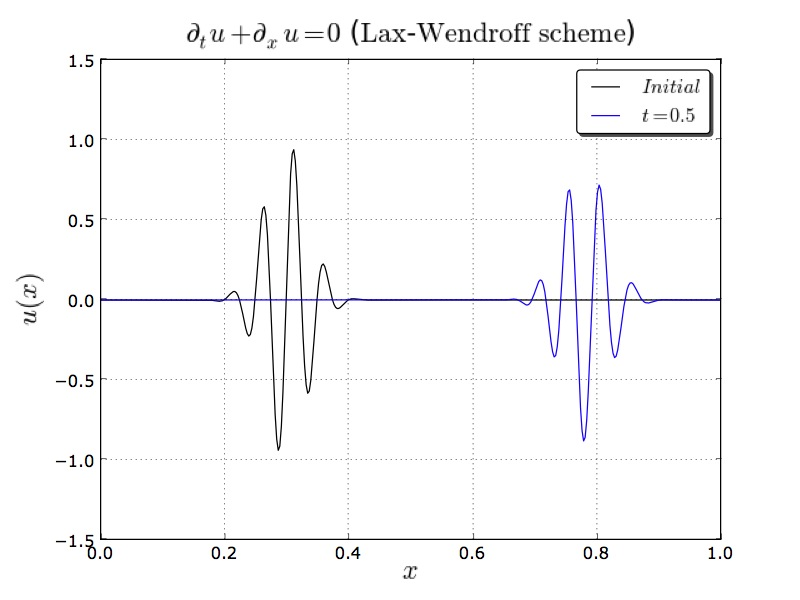
\includegraphics[width=10cm]{Images/cover.jpg}
	\end{center}
	\end{figure}

	\vskip10mm

	\begin{Large}
		\begin{table}[h]
		\centering
		\begin{tabular}{ll}
		%\hline
			{\bf \sc Author:}                   &  {\bf Nicolas LAMARQUE} \\
			{\bf \sc Date:}                        & {\bf August 2026}     \\
%\hline
		\end{tabular}
		\end{table}
	\end{Large}


	%\framebox{\epsfig{figure=.eps,height=70mm}}
	\vskip10mm

	\end{center}
\end{large}

\vskip20mm

\newpage


%------------------
% Abstract
\begin{abstract}
The purpose of this document is to recall some essential definitions of spectral analysis to evaluate difference approximations of the first-order wave equation. The concepts of dispersion relations and group velocities are first presented. Space and time Fourier analyses are successively described and their benefits are pointed out. Space analysis is available on infinite domains. It determines oscillation evolution, in terms of propagation velocities and amplitude changes, given a certain wavenumber. Time analysis is useful when there are interfaces such as mesh refinement or boundaries, to name a few. The roots of the so-called characteristic equation provide similar information as space Fourier transforms, except it is devoted to pulsations. This allows to introduce the notion of physical and spurious wave solutions. The Lax-Wendroff scheme is used as an illustration throughout this work.
\end{abstract}
%------------------

%------------------
% Mots-cles
\begin{keyword}
%% keywords here, in the form: keyword \sep keyword
Convection equation \sep Spectral analysis \sep Diffusion / Dispersion properties \sep Group velocities
\end{keyword}
%------------------

\end{frontmatter}
%--------------------------------------------------------------------------------------------------


%--------------------------
% Table des matieres
\tableofcontents
\newpage
%--------------------------


%--------------------------------------------------------------------------------------------------
% Section 1 - Dispersion relations
%==============================
\section{Introduction \label{sec:intro}}
%==============================
This document is devoted to the concept of dispersion relations and group velocities to study full discretizations. This kind of study is common for semi-discretizations \cite{Christon:2004,Vichnevetsky:1982}. In this work, $\Omega$ refers to the computational domain and $\Omega \subset \mathbb{R}^d$, with $d$ the number of dimensions. Transport phenomena in fluid are described by solving first-order hyperbolic partial differential equations (PDE). Other wave propagation from other disciplines (acoustics, electromagnetism, neutronics) can also be expressed as systems of first-order hyperbolic PDEs. The main focus is given to the most simple example of such equations: the linear convection equation. Moreover, the classical Lax-Wendroff (LW) scheme is used as the cornerstone of this report. \\

\noindent The linear convection equation reads:
\begin{equation}
\label{eq:conv_lin}
\ddt{u} + \bsa \cdot \nabla u = 0, 
\end{equation}

\noindent with $u=u(\bsx,t)$ the unknown, $\bsa$ the (constant) convective velocity. The exact solution of Eq.~(\ref{eq:conv_lin}) is:
$$ u(\bsx,t) = u_0(\bsx - \bsa t),$$

\noindent where $u_0(\bsx) = u(\bsx,0)$ is the initial solution. \\

\noindent In this document, we choose $d=1$ and $a>0$ for simplicity. The concepts, presented hereafter, can be generalized to $d>1$, but this introduces new difficulties like anisotropy, which will be mentioned elsewhere. Besides, the discretization of $\Omega$, noted $\mathcal{T}_h$, is made using regular elements, which leads to the mesh size $h = cst$. We note $U^n_j$ the solution of the discretization of Eq.~(\ref{eq:conv_lin}), at the discrete time $t^n = nk$, where $k$ is the time step, and associated with node (or control volume) located at $x_j = jh$. It approximates $u(x_j,t^n)$. The LW differencing scheme is written\cite{Leveque:2002}:
\begin{equation}
\label{eq:LW}
U_{j}^{n+1} = U_{j}^{n} - \frac{1}{2} c \left(U_{j+1}^{n} - U_{j-1}^{n}\right) + \frac{1}{2} c^2 \left(U_{j+1}^{n} - 2 U_{j}^{n} + U_{j-1}^{n}\right),
\end{equation}

\noindent which can be also written:

\begin{equation}
\label{eq:LW_carac}
Z U_{j}^{n}  = \left\{ I - \frac{c}{2} \left(E - E^{-1}\right) + \frac{1}{2} c^2 \left(E - 2I + E^{-1}\right) \right\} U_{j}^{n}, 
\end{equation}

\noindent where we have introduced the identity $I$, space- $E$ and time-shift $Z$ operators, and: \\
$$U_{j}^{n} = I U_{j}^{n}, \quad\quad  U_{j+1}^{n} = E U_{j}^{n},  \quad\quad U_{j}^{n+1} = Z U_{j}^{n}.$$

\noindent The CFL (Courant-Friedrichs-Lewy) number $c$ is used as a parameter to study the stability of the convection schemes and is defined by:
$$c = \frac{a k}{h} \, .$$

\noindent The LW scheme is second-order accurate both in space and time, and is $L^2 \ \mathrm{stable}$ provided $c \leq 1$ \cite{Hirsch:1988}. In the present document, we write: $\i = \sqrt{-1}$.
%--------------------------------------------------------------------------------------------------


%--------------------------------------------------------------------------------------------------
% Section 2 - Dispersion relations
%==============================
\section{Dispersion relations and definitions \label{sec:disper}}
%==============================
\noindent Equation (\ref{eq:conv_lin}) admits non-trivial plane-wave solutions of the form:
\begin{equation}
\label{eq:plane_wave}
u(x, t) = \exp(\i \xi x - \i \omega t) \, ,
\end{equation}


\noindent provided that the dispersion relation, which links the pulsation $\omega$ with the wavenumber $\xi$, 
\begin{equation}
\label{eq:DR}
\omega = \xi \, a,
\end{equation}

\noindent is respected \cite{Lighthill:1978,Trefethen:1996}. Identically, a discrete approximation of Eq.~(\ref{eq:conv_lin}) admits plane-wave solutions of the form:
\begin{equation}
\label{eq:disc_plane_wave}
U_j^n = \exp(\i \xi j h - \i \omega n k) \, ,
\end{equation}

Therefore, modified dispersion relations can be expressed. Injecting Eq.~(\ref{eq:disc_plane_wave}) in the difference schemes enables to write an expression, which links $\xi$ and $\omega$.

\vskip8mm

\begin{example}
The dispersion relation of the LW scheme can be obtained from:
\begin{equation}
\label{eq:tan_dispersion_relation_LW}
\tan{(\omega k)} = \frac{c \sin{(\xi h)}}{1- c^2 \left\{1-\cos{(\xi h)}\right\}}.
\end{equation}
\end{example}

\vskip8mm

\noindent As explained in \cite{Trefethen:1982}, as the grid is discrete, the dispersion relations like Eq.~(\ref{eq:tan_dispersion_relation_LW}) are multivalued and $2\pi$-periodic in $\xi h$ and $\omega k$. In practice and when needed, the relevant branch is chosen by continuity with the low-frequency limit $\omega k \sim c\,\xi h$. 
From Eq.~(\ref{eq:tan_dispersion_relation_LW}), it can be seen with the LW scheme, the dispersion relation related to a numerical scheme is a good approximation of Eq.~(\ref{eq:DR}) when $\xi h,\omega k \rightarrow 0$. On the other hand, it is also a formula involving trigonometric functions. Thus, the relation between $\xi$ and $\omega$ is no more linear and the scheme is said to be \emph{dispersive}. Indeed, essential propagation properties will depend on the pulsation or the wavenumber. 

\noindent The \emph{phase velocity} is the propagation speed of wave crests within a wave and is defined by:
\begin{equation}
\label{eq:phase_vel}
v_{\varphi}(\xi,\omega) = \frac{\omega}{\xi}.
\end{equation}

\noindent An even more important notion is the propagation velocity of energy, which is called \emph{group velocity} \cite{Lighthill:1978}: 
\begin{equation}
\label{eq:group_vel}
\mathcal{V}_{g}(\xi,\omega) = \frac{d\omega}{d\xi}.
\end{equation}

\noindent As Eq.~(\ref{eq:conv_lin}) is non-dispersive, those two velocities do not depend on $\xi$ or $\omega$ and are equal to the convection velocity $v_{\varphi} = \mathcal{V}_{g} = a$. Of course, this is not the case of most difference approximations. Dispersion errors imply that wavepacket components will not propagate at the same speed and will be gradually separated, leading to a (sometimes dramatic) shape deformation of the initial signal \cite{Trefethen:1996}.

\noindent It should be mentioned here that the group velocity theory is only valid for \emph{non-dissipative} media or in the limit of \emph{vanishing viscosity}, e.g for $\xi, \omega \in \mathbb{R}$. Any numerical diffusion introduces a frequency-dependent damping of Fourier components. The analysis is then more complicated. The wavepacket amplitude not only varies because of constructive/destructive interferences, but also due to diffusion. Nevertheless, when dispersion dominates, the predictions remain valid, at least for low frequencies \cite{Trefethen:1982}. 

\vskip8mm

\begin{example}
A general formula for the group velocity can be established by differentiating implicitly each side of (\ref{eq:tan_dispersion_relation_LW}) \cite{Sengupta:2004,Trefethen:1982,Trefethen:1996}:
$$ k \left(1 + \tan^2 (\omega k)\right) d\omega =  \frac{c h \cos (\xi h) d\xi}{1 - c^2 \left\{1-\cos (\xi h) \right\}} + \frac{c^3 h \sin^2 (\xi h) d\xi}{\left( 1 - c^2 \left\{1-\cos (\xi h) \right\}\right)^2}.
$$

\noindent Thus:
\begin{equation}
\label{eq:gen_group_vel_LW}
\mathcal{V}_{g}(\xi,\omega) = \frac{a}{1+\tan^2 (\omega k)} \left[\frac{\cos (\xi h)}{1 - c^2 \left\{1-\cos (\xi h) \right\}} + \frac{c^2 \sin^2 (\xi h)}{\left( 1 - c^2 \left\{1-\cos (\xi h) \right\}\right)^2} \right].
\end{equation}
\end{example}

\vskip8mm

\noindent Clearly, the relation between $\xi$ and $\omega$ is non-linear in Eq.~(\ref{eq:gen_group_vel_LW}). The interest of a formulae such as (\ref{eq:tan_dispersion_relation_LW}) and (\ref{eq:gen_group_vel_LW}) is also to treat separately the effects of space and time diffencing \cite{Trefethen:1982}. In what follows, however, we present other ways to derive dispersion relations and group velocities, which can be viewed as special cases of what has been presented so far. Their interest is that they are more common, rely on very well-known tools or introduce some concepts more easily, in the author's opinion. \\

\noindent The first one is based on \emph{space Fourier analysis} and \emph{the Cauchy problem} (\ref{eq:conv_lin}), e.g on an unbounded domain. Given a real wavenumber $\xi \in \mathbb{R}$ (an oscillation in space), one can determine the corresponding amplification factor, in the frame of the \emph{Von Neumann method} \cite{Hirsch:1988}. Then, a complex dispersion relation of the form: $\Sigma^{\star}(\xi) -\i \Omega^{\star}(\xi) \in \mathbb{C}$ can be deduced, where the $\star$ denotes the value provided by the numerical scheme. This first strategy is an efficient and classical tool in numerical analysis. It is often enough to get a good insight into a discretization. Nevertheless, for problems involving \emph{mesh refinement} or \emph{bounded domains}, a second analysis based on \emph{time Fourier transforms} has to be used and enables to introduce even more concepts \cite{Vichnevetsky:1982}. Another complex dispersion relation can also be written $M^{\star}(\omega) - i K^{\star}(\omega) \in \mathbb{C}$ in this case, with $\omega \in \mathbb{R}$.  


%--------------------------------------------------------------------------------------------------


%--------------------------------------------------------------------------------------------------
% Section 3 - Rappels sur les analyses en espace
%==============================
\section{Space Fourier transforms \label{sec:space}}
%==============================
We now study the main characteristics of numerical schemes, within the frame of space Fourier transforms. We suppose the domain $\Omega$ infinite, thus without boundaries. The problem associated with Eq.~(\ref{eq:conv_lin}) and the initial condition $u_0$ is a Cauchy problem.

%--------------
% sub 3.1
\subsection{Phase errors and propagation velocities}
Let us suppose that $U^n$ is a function with a finite norm, so that it can be expressed using Fourier transforms:
Let us suppose that the grid function $\{U_j^n\}_{j\in\mathbb{Z}}$ belongs to $\ell^2(\mathbb{Z})$, so that it admits the Fourier representation:
$$  U^n = \int_{-\infty}^{\infty} \widehat{U}^n(\xi) e^{\i \xi x} \frac{d\xi}{2\pi}, $$

\noindent with $\xi$ the wavenumber and $\i = \sqrt{-1}$. Then, applying a linear finite difference scheme leads, after some manipulations\footnote{Note that $E$ is a Toeplitz operator and $\hat{E}=e^{\i \xi h}$ \cite{Vichnevetsky:1982}}, to:
$$ U^{n+1}_j = \int_{-\infty}^{\infty} \widehat{U}^n(\xi) g(\xi) e^{\i \xi x_j} \frac{d\xi}{2\pi} .$$

\noindent where:
$$ g(\xi)=\frac{\widehat{U}^{n+1}(\xi)}{\widehat{U}^{n}(\xi)} $$
is the \emph{amplification factor} with the wavenumber $\xi$. On the other hand, the space Fourier transform of Eq.~(\ref{eq:conv_lin}) is:
\begin{equation}
\label{eq:conv_lin_Fourier}
\ddt{\widehat{u}} + \i \xi a \hat{u} = 0,
\end{equation}

\noindent and $\widehat{u}(t^{n+1})/\widehat{u}(t^{n}) = \exp \left(-\i \xi a k \right)$. As the dispersion relation of Eq.~(\ref{eq:conv_lin}) is $\omega = \Omega(\xi) = \xi a$, then the expression of the ideal amplification factor is: 
\begin{equation}
\label{eq:exact_g}
g^{ex}(\xi) = e^{- \i \omega k}
\end{equation}

\vskip8mm

\begin{example}
The amplification factor of the LW scheme (\ref{eq:LW}) is:
\begin{equation}
\label{eq:g_LW}
g^{LW}(\xi) = 1 - \i \ c \sin{(\xi h)} - c^2 \left\{1-\cos{(\xi h)}\right\}.
\end{equation}
\end{example}

\vskip8mm

\noindent As can be seen in Eq.~(\ref{eq:g_LW}), when a difference formula is used to approximate Eq.~(\ref{eq:conv_lin}), the pulsation of a harmonic $\xi$ is only an approximation of the real one. Moreover, because in the general case, the difference approximation introduces spurious diffusion. Then, the amplicafication factor of a numerical scheme can be written:
\begin{equation}
\label{eq:g}
g(\xi) = e^{s^{\star} k} = e^{\sigma^{\star}k - \i \omega^{\star} k}.
\end{equation}

\noindent Equation~(\ref{eq:g}) then allows to write the functional: 
$$ \begin{array}{rcl}
   S^{\star}:\mathbb{R} &\longrightarrow& \mathbb{C} \\
   \xi &\longmapsto& S^\star(\xi)=\sigma^\star(\xi)-i\,\omega^\star(\xi) \, , 
   \end{array}
$$

\noindent which definies the \emph{modified dispersion relation} of the difference scheme. $\omega^{\star}$ is to be compared with the real pulsation and holds the \emph{phase errors}, while $\sigma^{\star}$ is linked with the \emph{numerical diffusion} of the scheme. We can also define the modified wavenumber \cite{Hirsch:1988}:
\begin{equation}
\label{eq:kstar}
\xi^{\star}(\xi) = \frac{\Omega^{\star}(\xi)}{a} ,
\end{equation}

\noindent and the modified phase velocity: 
\begin{equation}
\label{eq:phase_vel_star}
v_{\varphi}^{\star}(\xi) = \frac{\Omega^{\star}(\xi)}{\xi} .
\end{equation}

\noindent Furthermore, a cut-off wavenumber can be defined as the largest accurately represented wavenumber, which can be represented by the discretization\footnote{The phase error at $\xi=\xi_c$ is often big (up to 50\%). Another definition must be written to better evaluate phase accuracy. See \cite{Bailly:2004}.} and is often far smaller than $\pi / h$:
$$ \xi_c h = \max_{\xi h} \left( \xi^{\star} h \right).$$

\vskip8mm

\begin{example}
\noindent The modified dispersion relation of the LW scheme gives:
\begin{equation}
\label{eq:omegastar_LW}
\omega^\star = \frac{1}{k} \arctan \left( \frac{c \sin{(\xi h)}}{1- c^2 \left\{1-\cos{(\xi h)}\right\}}\right).
\end{equation}

\noindent Then, its modified wavenumber is:
\begin{equation}
\label{eq:kdx_LW}
\xi^{\star} h = \frac{1}{c} \arctan{\left[\frac{c \sin{(\xi h)}}{1- c^2 \left\{1-\cos{(\xi h)}\right\}}\right]}.
\end{equation}
\noindent Figure~(\ref{fig:kdx_lw}) shows the modified wavenumber of the LW scheme for different CFL numbers. The LW scheme has a good phase accuracy for longer wavelengths, but shows a poor behavior for badly resolved scales, especially for small CFL numbers. It is noteworthy that the LW scheme has no phase error\footnote{No error at all in fact !} at $c=1$. Table~(\ref{tab:kdx_lw}) gathers the cut-off wavenumbers (and the corresponding wavelengths $\lambda=2\pi /\xi$) of the LW scheme, depending on the CFL number. Moreover, wavenumbers $k_a h$, such that:
$$ \left|\xi^{\star}(\xi_a)-\xi_a\right|/\xi_a < 0.01$$
are also added in Tab.~(\ref{tab:kdx_lw}), to assess the phase accuracy.
\end{example}

\begin{figure}[h!]
\centering
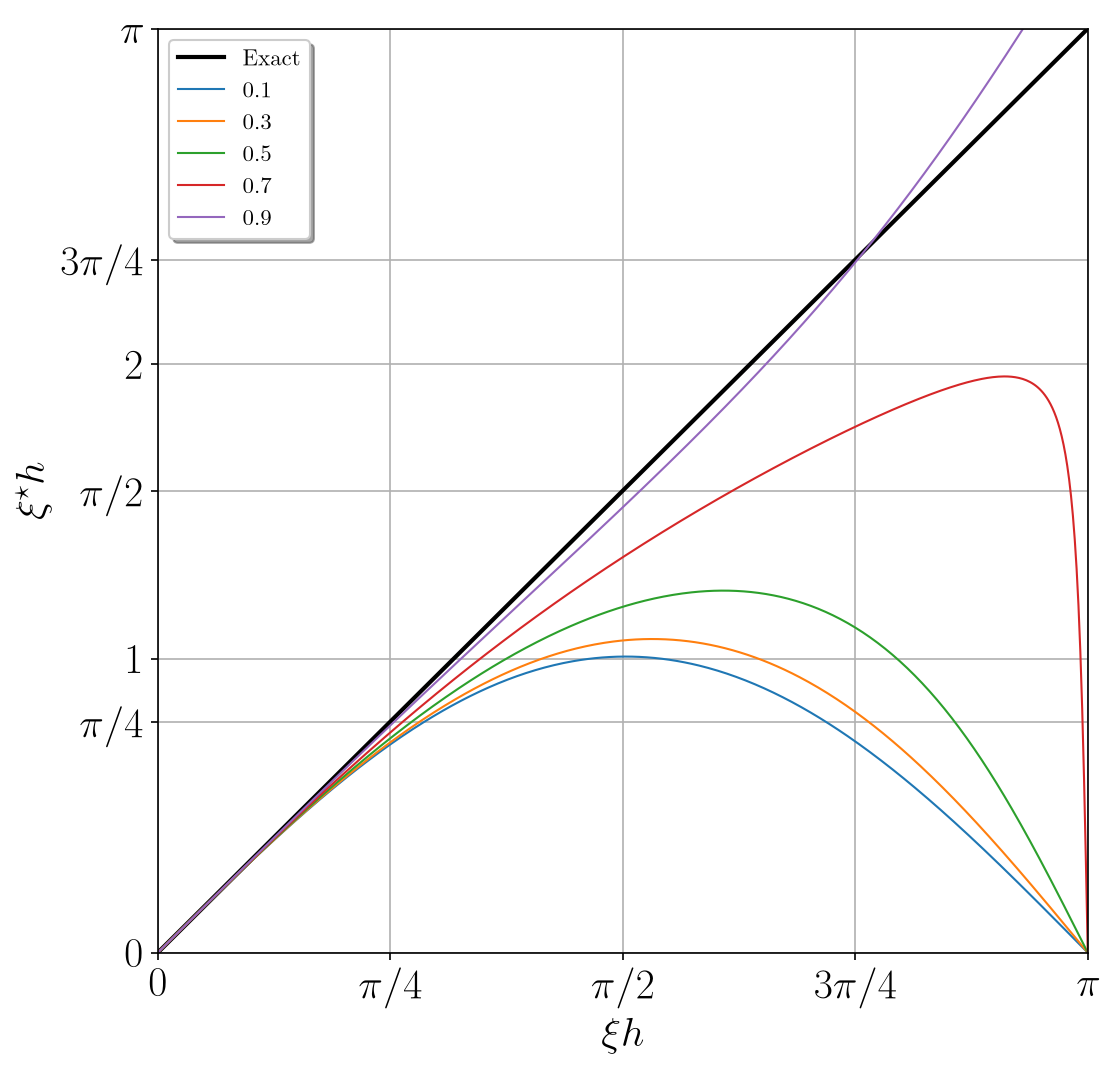
\includegraphics[width=80mm]{Images/kdx_lw.png}
\caption{Modified wavenumber of the LW scheme for CFL from $0.1$ to $0.9$.}
\label{fig:kdx_lw}
\end{figure}

\begin{table}[ht!]
\begin{center}
%\begin{tabular}{p{15mm}||p{15mm}|p{15mm}||p{15mm}|p{15mm}}
\begin{tabular}{c||c|c||c|c}
$c$ & $\xi_c h$ & $\lambda_c / h$ & $ \xi_a h$ & $\lambda_a / h$\\
\hline
$0.1$ & $1.007$ & $6.24$ & $0.245$ & $25.6$ \\
$0.3$ & $1.066$ & $5.89$ & $0.251$ & $25.0$ \\
$0.5$ & $1.231$ & $5.10$ & $0.283$ & $22.2$ \\
$0.7$ & $1.959$ & $3.21$ & $0.346$ & $18.2$ \\
$0.9$ & $\mathit{3.491}$ & $\mathit{1.80}$ & $0.591$ & $10.6$ \\
\end{tabular}
\end{center}
\caption{$\xi_c h$ and $\xi_a h$ for the LW scheme and different CFL numbers.}
\label{tab:kdx_lw}
\end{table}

\noindent Table~(\ref{tab:kdx_lw}) confirms that phase errors are lower when $c\rightarrow 1$. It also shows that $\xi^{\star}$ is relatively small, compared with $\pi$ (the supposedly maximum non-dimensionalized wavenumber), which is linked with the strong discrepencies of the scheme with small wavelengths. Phase errors are bigger than $1\%$, as soon as the wavelength is smaller than around $20 h$, for a large band of CFL numbers ($c<0.5$). This shows that dispersion errors are non-negligible, even when resolution seems rather correct (15-20 nodes per wavelength).

\vskip8mm

\noindent As said in section~\ref{sec:disper}, group velocity can be used to further describe wave packets and energy transport. Knowing the modified pulsation, the group velocity of the numerical scheme can be calculated in the same way as the exact one:
\begin{equation}
\label{eq:vgroup_star}
\mathcal{V}^{\star}_g (\xi) = \frac{d \omega^{\star}}{d\xi} = a \frac{d\xi^{\star}}{d\xi}.
\end{equation}

\noindent Depending on the resolution power of the difference schemes, some waves can have an unexpected behavior. Group velocity is the main tool to discriminate those waves, as it gives information about the way they propagate. The longer wavelenghts ($\xi h \rightarrow 0$) behave like physical waves (consistency condition) and moves in the right direction, at the right velocity and dispersion errors are relatively small, especially when a high-order scheme is used. On the other hand, the smaller wavelengths ($\xi h \rightarrow \pi$), which are badly resolved (only few points), are moving at a wrong speed, in the opposite direction. They can be considered as spurious waves, as they do not follow the physical laws and can threaten the stability of the computation. Several illustrations are provided in \cite{Trefethen:1982,Vichnevetsky:1982}. Vichnevetsky and Bowles \cite{Vichnevetsky:1982} have called the first oscillations {\it p-waves} and the spurious ones {\it q-waves}.

\noindent A good criterion to distinguish waves is thus the sign of the group velocity:

\begin{definition}
\noindent If the product $a \, \mathcal{V}^{\star}_g < 0$, then the corresponding wave $\xi$ is a spurious one, which is called {\it q-wave}.
\end{definition}

\vskip8mm

\noindent {\it q-waves} can be very dangerous, as they carry some energy in the wrong direction or be stationary, can reflect on boundaries and eventually lead to numerical instabilities \cite{Trefethen:1982,Vichnevetsky:1982}.

\begin{example}
\noindent The modified group velocity of the LW scheme is:
\begin{equation}
\label{eq:vgroup_LW}
\frac{\mathcal{V}^{\star}_g}{a} = \frac{(1-c^2) \cos{(\xi h)} + c^2}{c^2 \sin^2 (\xi h) + \left\{c^2 \cos (\xi h) - c^2 +1 \right\}^2},
\end{equation}
\noindent and Figure~(\ref{fig:vg_lw}) displays it for different CFL numbers. As explained above, the scheme behaves rather well for $\xi h \rightarrow 0$, especially for higher CFL numbers. In general, phase errors are very significant when $\lambda \approx 10-20 h$. When oscillations are smaller than around $4 h$, they are even convected in the wrong direction (especially when the CFL number is small). One should also note that there are no {\it q-waves} at higher CFL numbers (see $c=0.9$).
 \end{example}

\begin{figure}[h!]
\centering
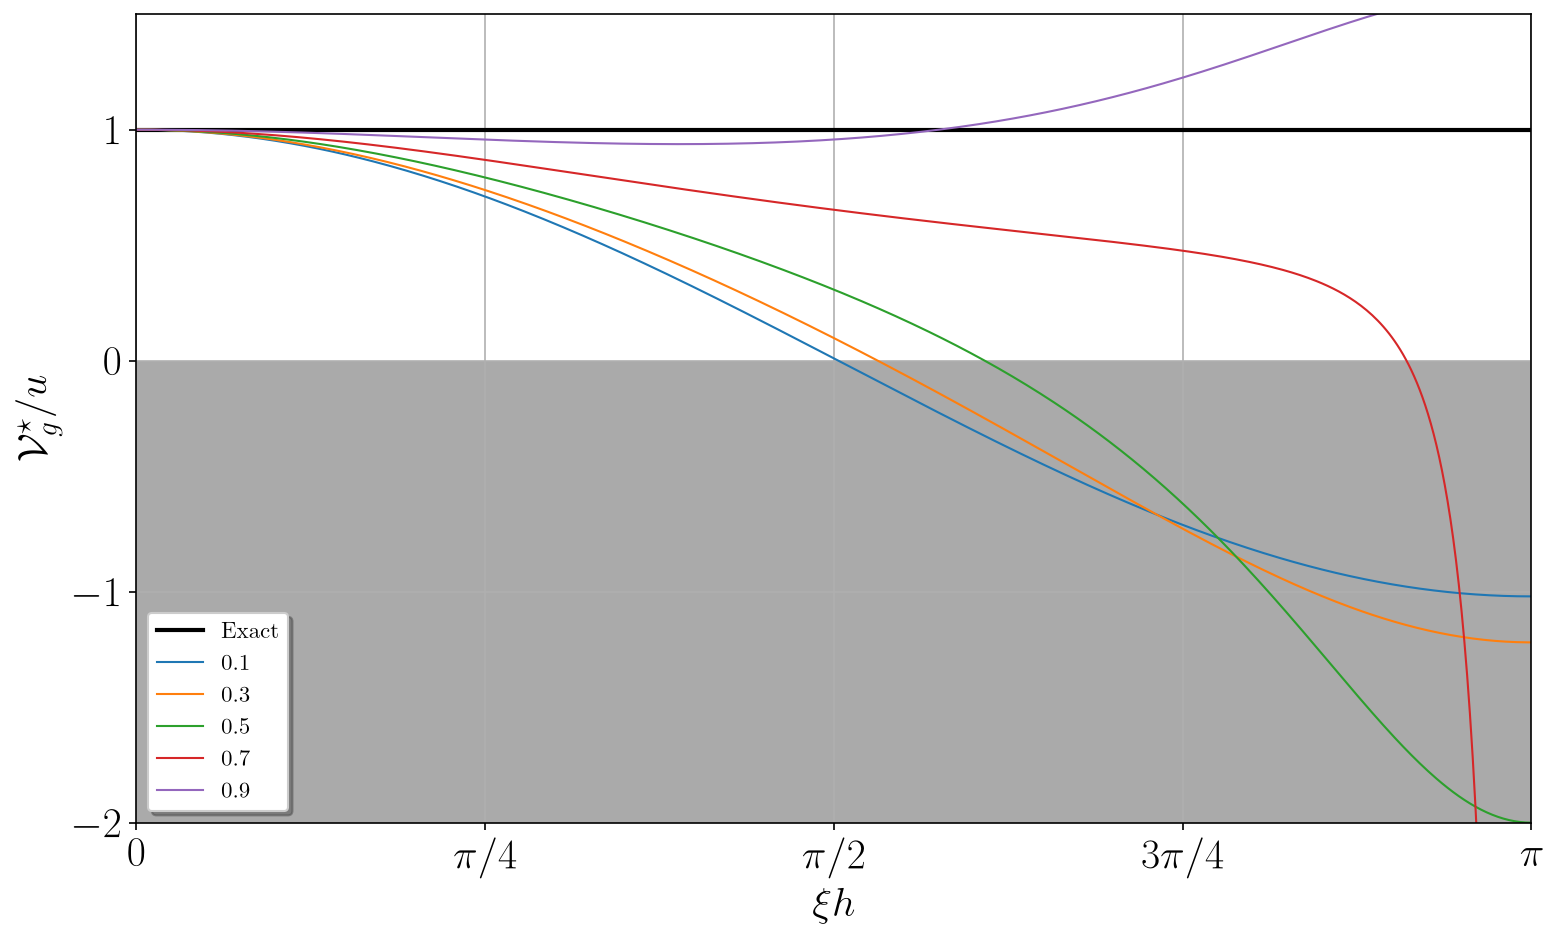
\includegraphics[width=120mm]{Images/vg_lw.png}
\caption{Modified group velocity of the LW scheme for CFL from $0.1$ to $0.9$. The shaded area corresponds to negative group velocity waves (spurious waves).}
\label{fig:vg_lw}
\end{figure}
%--------------

%--------------
% sub 3.2
\subsection{Diffusion errors}
So far, we have only considered phase errors, but most numerical schemes also introduce diffusion errors, as soon as $\Sigma^{\star}$ is not zero. Indeed, we have:
\begin{equation}
\label{eq:ampli_imomega}
\left|g(\xi) \right| = \exp \left(\sigma^{\star} k\right).
\end{equation}

\noindent Consequently:
\begin{itemize}
 \item if $\exists ~\xi \mathrm{~such~that~} \sigma^{\star} > 0$, the method is unstable (exponential growth),
 \item if $\sigma^{\star} = 0$, the method is non-dissipative or marginally stable,
 \item if $\exists ~\xi \mathrm{~such~that~} \sigma^{\star} < 0$, the method is dissipative.
\end{itemize}

\noindent Numerical diffusion implies a decay of wave amplitudes and a smearing of strong gradients. This phenomenon is usually not desirable, for example to simulate turbulence. Nevertheless, it tends to stabilize a numerical method and often eliminates spurious waves, generated by phase errors, the Gibbs phenomenon, or spurious reflections at interfaces (mesh refinement, boundaries...). However, we recall that the group velocity theory only works in the limit of zero or vanishing viscosity \cite{Trefethen:1982}. Indeed, the amplitude decay is due to two phenomena: diffusion and destructive interferences due to dispersion. Therefore, the amplification factor should just be used to study numerical diffusion of sine waves.

\vskip8mm

\begin{example}
Figure~(\ref{fig:ampli_lw}) displays the amplification factor modulus of the LW scheme for different CFL numbers. For small CFL numbers, the LW is hardly dissipative, even for high wavenumbers. As $c \rightarrow \sqrt{2}/2$, numerical diffusion gets stronger, especially for $\xi h \rightarrow \pi$. Then, as $c \rightarrow 1$, the scheme is again less dissipative. It is stable for $c\le 1$. As an example, Fig.~(\ref{fig:ampli_lw}) shows $\left|g(\xi)\right|$ for $c=1.1$, which belongs to the unstable region and leads to the simulation blow-up.
 \end{example}

\vskip8mm

\begin{figure}[h!]
\centering
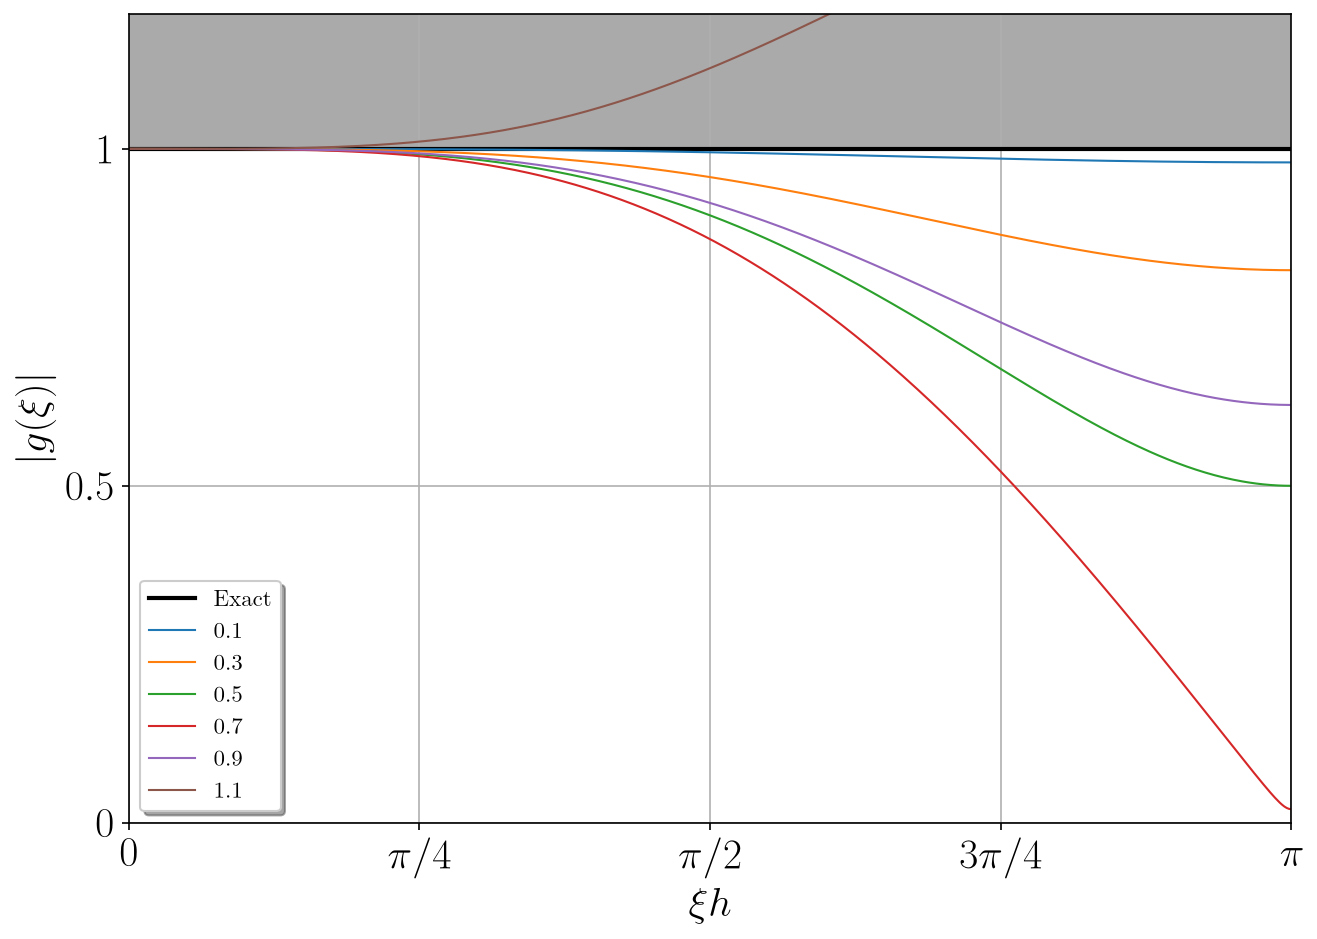
\includegraphics[width=120mm]{Images/ampli_lw.png}
\caption{Amplification factor modulus of the LW scheme for CFL from $0.1$ to $1.1$. The shaded area corresponds to the unstable region.}
\label{fig:ampli_lw}
\end{figure}
%--------------


%--------------------------------------------------------------------------------------------------


%--------------------------------------------------------------------------------------------------
% Section 4 - Rappels sur les analyses en temps
%==============================
\section{Time Fourier transforms \label{sec:time}}
%==============================
We have shown that space Fourier transforms are very useful to study wave propagation within the frame of the Cauchy problem (initial value problem with infinite domains). Despite the power of this tool, it remains difficult to analyze what happens next to boundaries or interfaces. To fix this problem, Vichnevetsky proposes to work with time Fourier transforms \cite{Vichnevetsky:1982}.

%--------------
% sub 4.1
\subsection{Characteristic equation and dispersion relations}
Let suppose that $U_j$ is a function with a finite norm, so that it can be expressed using (discrete) time Fourier transforms:
$$  U^n_j = \int_{-\pi/k}^{\pi/k} \breve{U}_j(\omega) e^{\i \omega n k} \frac{d\omega}{2\pi}, $$

\noindent and:
$$ \breve{U}_j(\omega) = k \sum_{-\infty}^{+\infty} U^n_j e^{-\i \omega n k }.$$

\noindent Following the methodology of \cite{Vichnevetsky:1982} and using the time Fourier transform\footnote{It is worth recalling $\breve{Z}=e^{\i \omega k}$.}, the \emph{characteristic equation} of a difference scheme can be obtained:
$$ f(c,\omega k,\breve{E},\breve{E}^2,\breve{Z},\dots ) = 0.$$

\noindent The characteristic equation has generally \emph{several roots} $\breve{E}_{\alpha}$ and the time Fourier transform of the solution is composed with several components:
$$  \breve{U}_j (\omega) = \sum_{\alpha} \breve{\phi}_{j,\alpha}(\omega) = \sum_{\alpha} \breve{\phi}_{0,\alpha} \left[\breve{E}_{\alpha}(\omega)\right]^j, $$


\noindent Using time Fourier transforms, Eq.~(\ref{eq:conv_lin}) can also be rewritten:
\begin{equation}
\label{eq:conv_lin_time}
\i \omega \breve{u} + a \ddx{\breve{u}} = 0,
\end{equation}

\noindent Then $\breve{u}(x_{j+1})/\breve{u}(x_{j})=\exp \left(-\i \omega x / a\right)$. As the dispersion relation of Eq.~(\ref{eq:conv_lin}) is $\xi=K(\omega)=\omega / a$, then the exact space-shift operator\footnote{Sometimes called \emph{space} amplification factor.} is $\breve{E}^{ex} = \exp \left(-\i \xi h \right)$.

\noindent Similarly to the work done with space Fourier transforms, we can introduce \emph{modified pulsation, wavenumber, phase and group velocities}, writting:
\begin{equation}
\label{eq:E_omega}
\breve{E}(\omega) = e^{\tau^{\star} h} = e^{\mu^{\star}h -\i \ \xi^{\star} h}.
\end{equation}

\noindent Eq.~(\ref{eq:E_omega}) allows to write a functional:
$$ \begin{array}{rcl}
   K^{\star}:\mathbb{R} &\longrightarrow& \mathbb{C} \\
   \omega &\longmapsto& T^{\star}(\omega) = M^{\star}(\omega) - i K^{\star}(\omega) = \mu^{\star}- \i \xi^{\star}, .    
   \end{array}
$$

\noindent which is the dispersion relation of the root $\breve{E}$. By analogy with section~\ref{sec:space}, $\xi^\star$ is to be compared with the real wavenumber and holds \emph{the phase errors} of the scheme, while $\Im \left(\xi^\star \right)$ is linked with the numerical diffusion. Therefore, the real part of $K^{\star}$ is the modified dispersion relation.

\noindent The modified dispersion relation also leads to the definitions:
\begin{eqnarray}
\label{eq:kstar_omega}
\omega^{\star} (\omega) &=& K^{\star}(\omega) a = - \frac{a}{h} \arctan\left(\frac{\Im (\breve{E})}{\Re (\breve{E})}\right) \\
\label{eq:vphi_omega}
v_{\varphi}^{\star}(\omega) &=& \omega / K^{\star}(\omega) = - \frac{a \omega k}{c} \left\{\arctan\left(\frac{\Im (\breve{E})}{\Re (\breve{E})}\right)\right\}^{-1} \\
\label{eq:vg_omega}
\mathcal{V}^{\star}_{g}(\omega) &=& \frac{a}{(\partial \omega^{\star} / \partial \omega)}.
\end{eqnarray}

\noindent From relation (\ref{eq:kstar_omega}), one can also calculate wavelengths associated with a pulsation $\omega$:
$$\lambda^{\star}(\omega) = \frac{2 \pi}{K^{\star}(\omega)} .$$

\vskip8mm

\begin{example}
Using the methodology described above, the LW scheme (\ref{eq:LW}) becomes:
$$ \breve{Z} = 1 - \frac{c}{2} \left(\breve{E} - \breve{E}^{-1} \right) + \frac{c^2}{2} \left(\breve{E} -2 +\breve{E}^{-1} \right). $$

\noindent This leads to the characteristic equation of the LW scheme:
\begin{equation}
\label{eq:LW_eq_carac}
\breve{E}^2 + \underbrace{\frac{2\left(1-c^2-\breve{Z}\right)}{c(c-1)}}_{b(\omega)} \breve{E} + \frac{c+1}{c-1} = 0.
\end{equation}

\noindent The roots of Eq.~(\ref{eq:LW_eq_carac}) are:
$$ \breve{E}_{p/q} = \frac{-b(\omega) \pm \sqrt{\Delta(\omega)}}{2},$$

\noindent with:
$$ \Delta(\omega) = {b(\omega)}^2 - 4 \ \frac{c+1}{c-1}.$$

\noindent It means there is two kind of waves, which can propagate and the time Fourier transform of the solution is:
$$ \breve{u}_j (\omega) = \breve{p}_j (\omega) + \breve{q}_j (\omega),$$

\noindent such that:
$$\begin{array}{ccc}
   \breve{p}_j &=& \breve{p}_0 \left[\breve{E}_{p}\right]^j \\
   \breve{q}_j &=& \breve{q}_0 \left[\breve{E}_{s}\right]^j \\
  \end{array}
$$
\end{example}

\vskip8mm

\noindent In comparison with the space Fourier transforms, the main advantage is to highlight that there exists several waves associated with the scheme. For instance, in the case of the LW scheme, there are two waves for a given pulsation $\omega$. This is due to the fact that a three-point explicit scheme has a quadratic characteristic equation. The first one, corresponding to the well-resolved wavenumbers, are named {\it p-waves} or physical / smooth waves. Their group velocity is such that $a~\mathcal{V}_g^{\star} > 0$. On the other hand, there are also badly-resolved harmonics and can be called {\it q-waves} or spurious / saw-tooth waves. Their group velocity is such that $a~\mathcal{V}_g^{\star} < 0$. Thus, they propagate upstream, which is wrong and explains their name. As in the case of space analysis, we can introduce the definitions:

\begin{definition}
\label{def:root}
\noindent Considering a root $\breve{E}$, when $\omega k \rightarrow 0$:
\begin{itemize}
\item if $a~\mathcal{V}_{g}^{\star} > 0$, then the root is a {\it p-wave}.
\item if $a~\mathcal{V}_{g}^{\star} < 0$, then the root is a {\it q-wave}. 
\end{itemize}
\end{definition}

\vskip8mm

\noindent This definition is to be carefully used when the difference approximation is dissipative, as it is discussed in paragraph~\ref{sec:cutoff}.

\vskip8mm

\begin{example}
\noindent Figures~(\ref{fig:lw_omega}), (\ref{fig:lw_lambdastar_omega}) and (\ref{fig:lw_vgtime}) display an example of modified pulsation, wavelenghts and group velocities for the LW scheme for a CFL number of $c=0.1$. Again, there is two solutions for a given pulsation. As far as the {\it p-wave} is concerned, the LW scheme has a satisfactory behavior for smaller pulsations. $\omega^{\star}$ is close to $\omega$, waves are well-represented ($\lambda^{\star} \approx \lambda$) and propagate at the right velocity ($\mathcal{V}_g^{\star} / a \rightarrow 1$). At the same time, the {\it q-wave}, badly-resolved (close to $2h$), also exists for the same pulsations and propagate in the opposite direction. As pulsation goes bigger, phase errors are more sensible and the behavior of both waves gets closer.

\begin{figure}[h!]
\centering
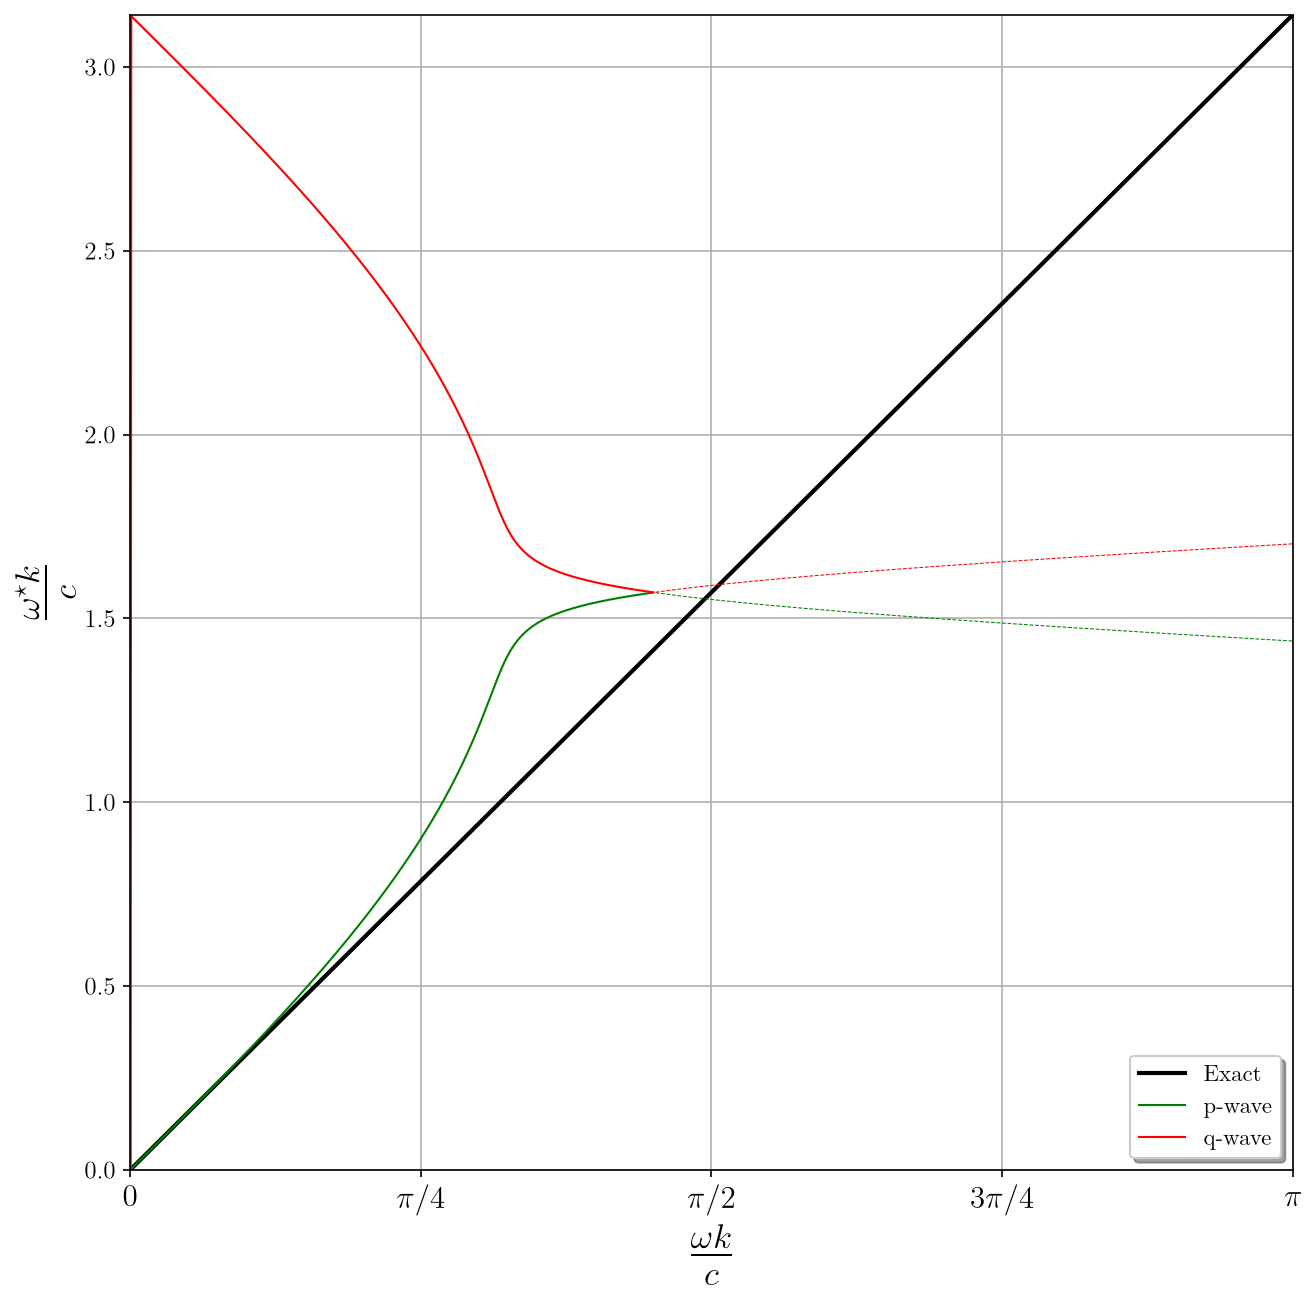
\includegraphics[width=100mm]{Images/lw_tf_omega.png}
\caption{Modified pulsations of the LW scheme depending on the pulsation $\omega$. Black line: exact. Green line: {\it p-waves}. Red line: {\it q-waves}. CFL number is $c=0.1$. Dashed lines are, in this case, evanescent solutions.}
\label{fig:lw_omega}
\end{figure}

\begin{figure}[h!]
\centering
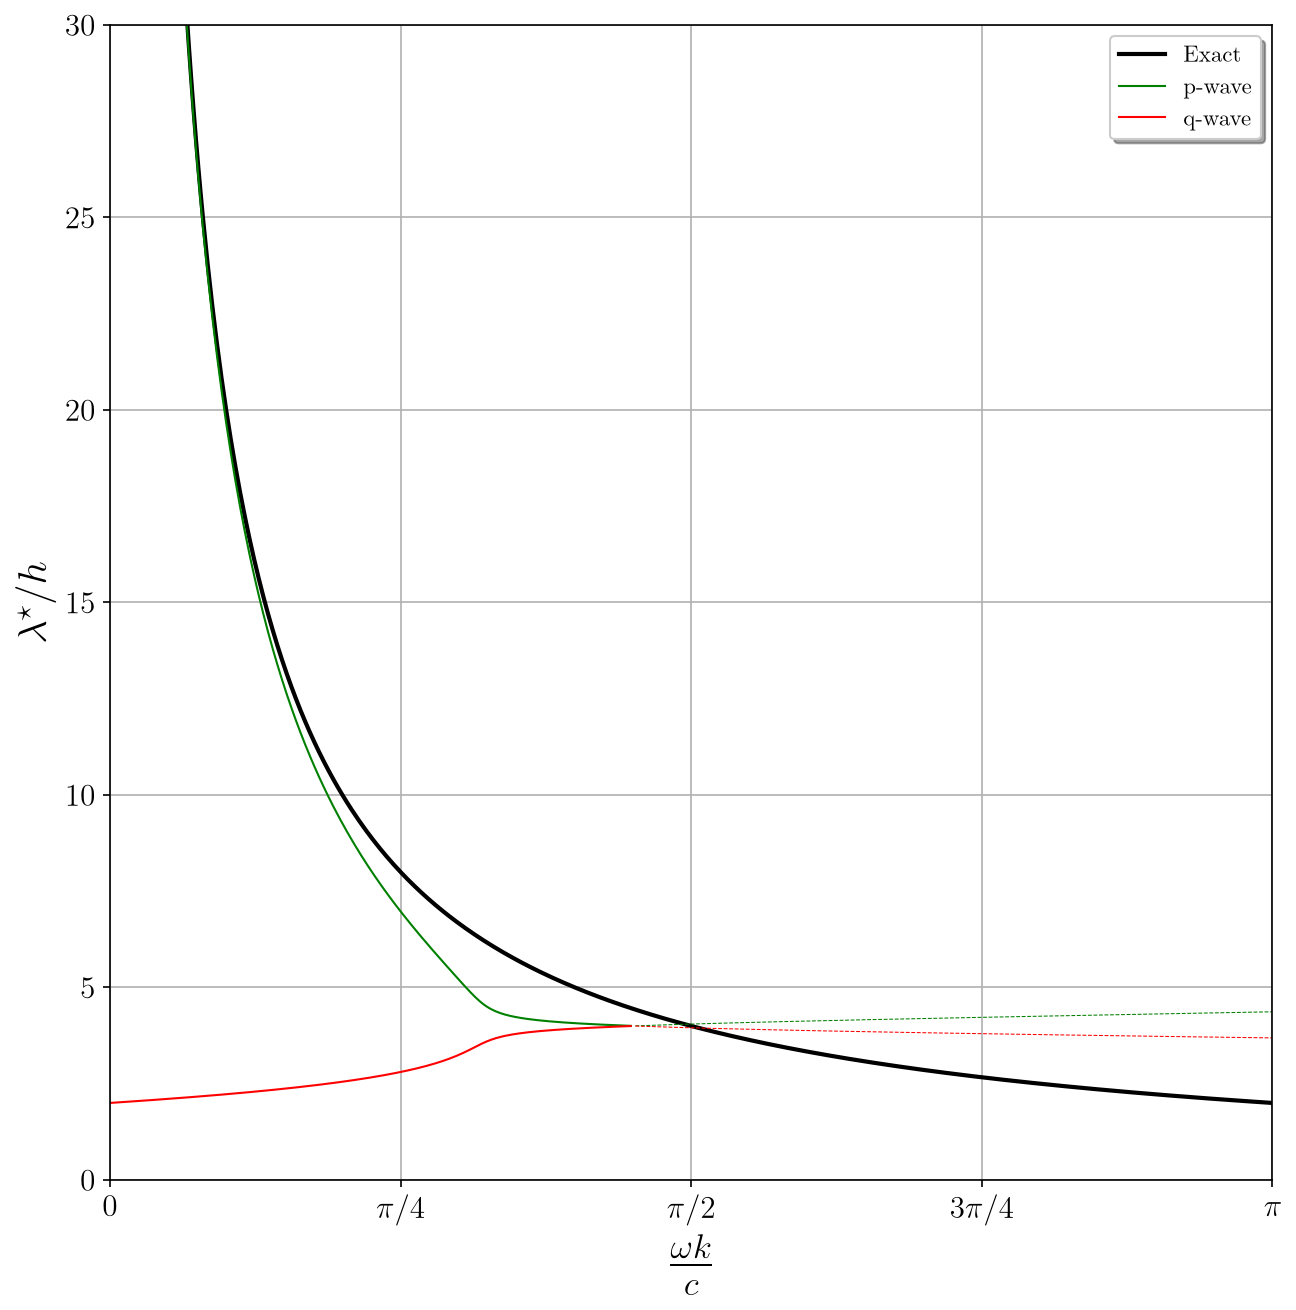
\includegraphics[width=100mm]{Images/lw_tf_lambda.png}
\caption{Modified wavelenghts of the LW scheme depending on the pulsation $\omega$. Black line: exact. Green line: {\it p-waves}. Red line: {\it q-waves}. CFL number is $c=0.1$. Dashed lines are, in this case, evanescent solutions.}
\label{fig:lw_lambdastar_omega}
\end{figure}

\begin{figure}[h!]
\centering
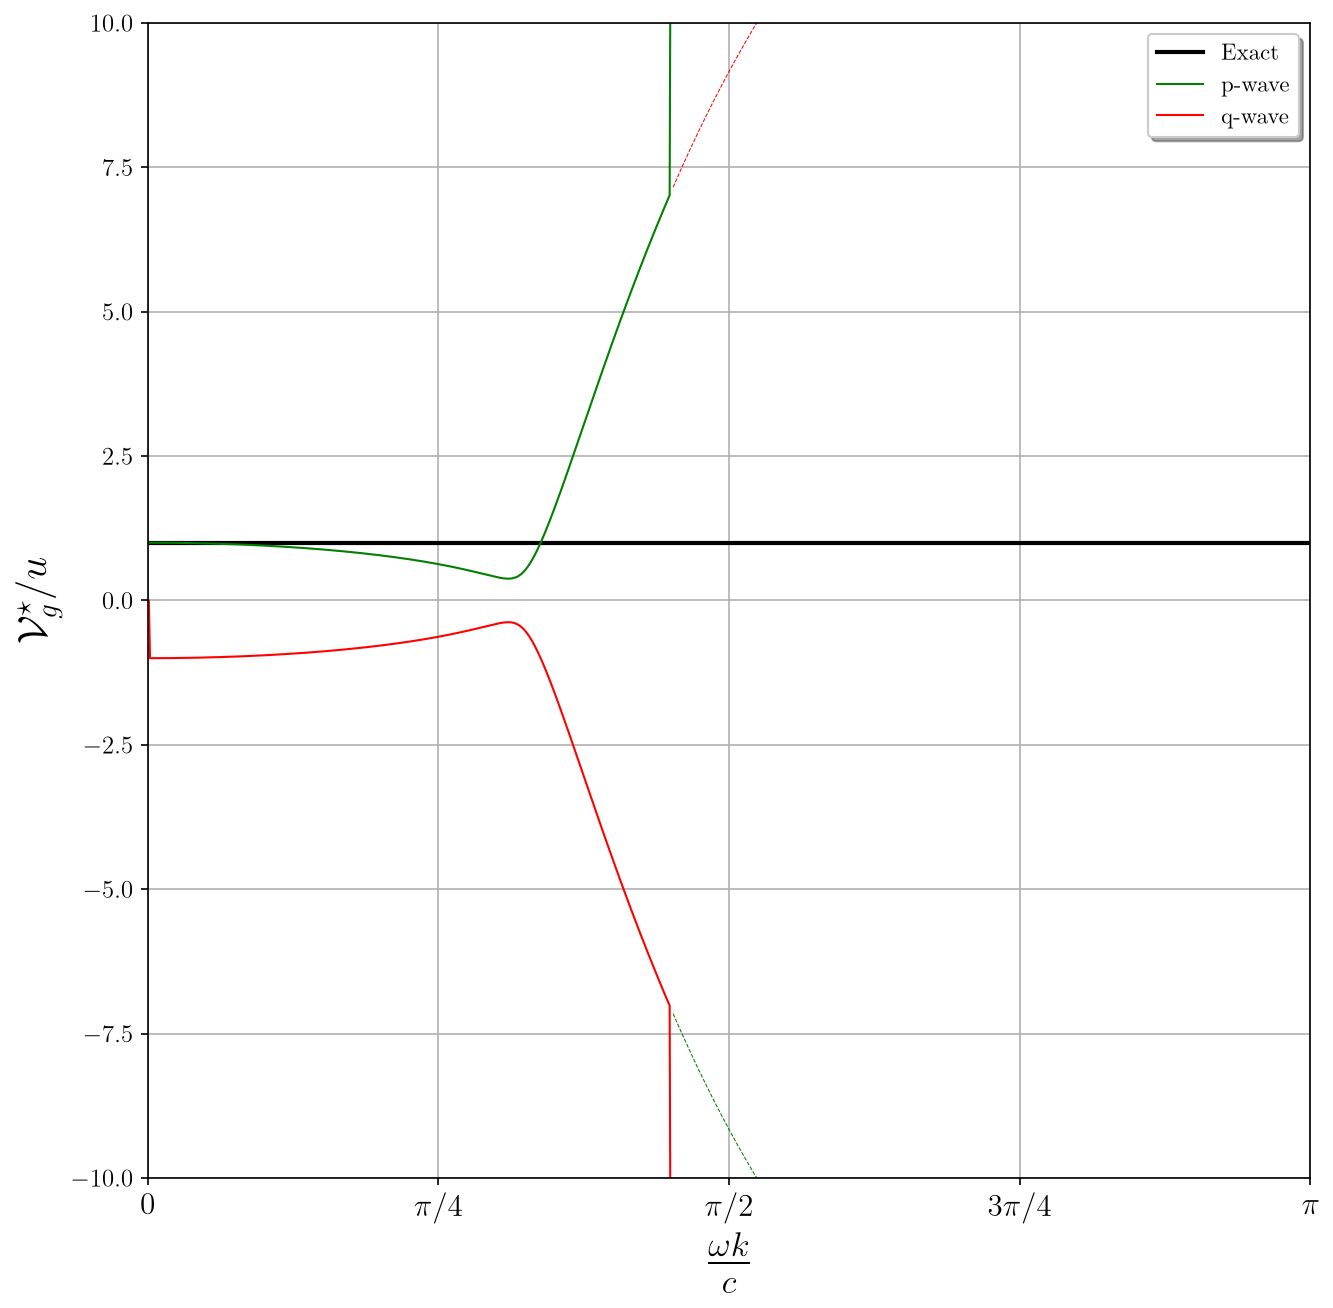
\includegraphics[width=100mm]{Images/lw_tf_vg.png}
\caption{Modified group velocities of the LW scheme depending on the pulsation $\omega$. Black line: exact. Green line: {\it p-waves}. Red line: {\it q-waves}. CFL number is $c=0.1$. Evanescent solutions do not appear on screen.}
\label{fig:lw_vgtime}
\end{figure}

\end{example}

%--------------

%--------------
% sub 4.2
\subsection{Diffusion errors}
As mentionned in section~\ref{sec:space}, most numerical schemes introduce diffusion errors. Indeed, as soon as $\mu^{\star}$ is not zero, the corresponding root is diffused or anti-diffused.
\noindent Suppose that $a>0$. If $u~\mathcal{V}^{\star}_{g}$ is positive, this is a physical wave and:
\begin{itemize}
\item $\mu^{\star} = 0$, the scheme is non-dissipative.
\item if $\exists ~\omega$ such that $\mu^{\star} > 0$, the scheme is unstable.
\item if $\exists ~\omega$ such that $\mu^{\star} < 0$, the scheme is dissipative.
\end{itemize}

\noindent Inversely, if $a~\mathcal{V}^{\star}_{g}$ is negative, this is a spurious wave. Then it moves in the wrong direction and:
\begin{itemize}
\item $\mu^{\star} = 0 = 0$, the scheme is non-dissipative.
\item if $\exists ~\omega$ such that $\mu^{\star} = 0 < 0$, the scheme is unstable.
\item if $\exists ~\omega$ such that $\mu^{\star} = 0 > 0$, the scheme is dissipative.
\end{itemize}

\begin{example}
Figure~(\ref{fig:mod_lw}) shows the modulus of the LW scheme characteristic equation roots $\breve{E}_{p/s}$ for a CFL number $c=0.1$. Using Fig.~(\ref{fig:lw_lambdastar_omega}), we can see that the smooth waves are slowly diffused, until $\lambda \approx 5-10 h$.  On the other hand, all the spurious waves (red line) are diffused at this CFL number. Beyond a cut-off frequency $\omega k / c \approx 1.4$, solutions are very rapidly dissipated and are refered as evanescent solutions (dashed lines on the figures).
\end{example}

\vskip8mm

\begin{figure}[h!]
\centering
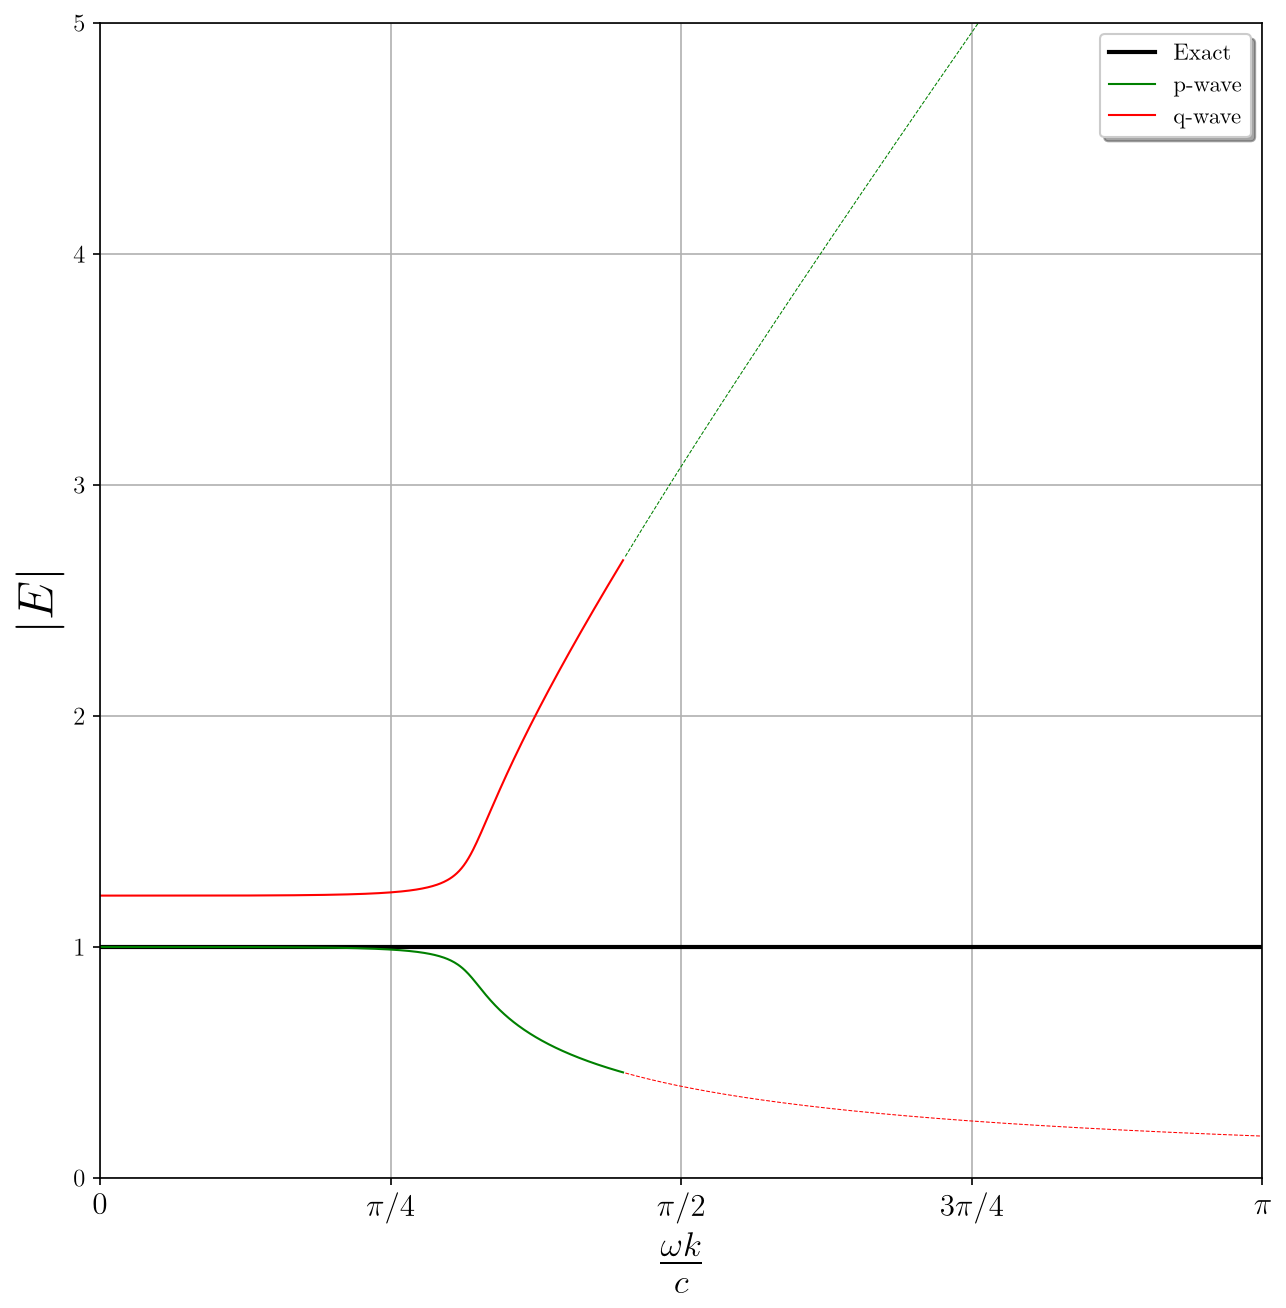
\includegraphics[width=100mm]{Images/lw_tf_abs.png}
\caption{Roots modulus of the LW scheme characteristic equation, depending on the pulsation $\omega$. Black line: exact. Green line: {\it p-waves}. Red line: {\it q-waves}. CFL number is $c=0.1$. Dashed lines are evanescent solutions.}
\label{fig:mod_lw}
\end{figure}

%--------------

%--------------
% sub 4.3
\subsection{Evanescent solutions and cut-off frequency \label{sec:cutoff}}
\noindent We finally give a brief discussion about evanescent solutions and the definition of {\it p-} and {\it q-waves}. Using LW as the reference, we only consider difference scheme with a quadratic characteristic equation, but this can be generalized for higher-order equations.

\noindent In the examples given above (see Figs.~(\ref{fig:lw_omega})-(\ref{fig:lw_vgtime})), some part of the solutions are indicated with dashed lines. Going from a continuous to a dash line corresponds to a rapid change of behavior, as $\omega k / c$ grows. The sign of group velocity changes, $|E|$ goes from a value bigger ({\it resp.} smaller) to a value smaller ({\it resp.} bigger) than 1. This change occurs at the same value of $\omega k / c$ for both roots\footnote{In the case of a quadratic characteristic equation.}. The dashed part of the roots of Eq.~(\ref{eq:LW_eq_carac}) are strongly damped for $c=0.1$. It is then straightforward to define a cut-off frequency $\omega ~|~\omega^{\star}_p = \omega^{\star}_q$. Pulsating at a frequency beyond this limit results in no wave in the domain. This phenomenon is even clearer with a non-dssipative scheme, as highlighted by Vichnevetsky and Bowles \cite{Vichnevetsky:1982}, for the second-order centred scheme. In such a case, solutions are evanescent beyond the cuf-off frequency. Those similar behaviors are not surprising as the LW scheme is hardly dissipative and close to the second-order centred scheme, for $c \rightarrow 0$. 

\noindent For higher CFL numbers, conclusions are somewhat different, in the case of diffusive schemes, like LW. They remain roughly the same for {\it p-waves} ($a ~\mathcal{V}_{g}^{\star} > 0$ and $\left| E_p\right| \rightarrow 1^-$ for $\omega k / c \rightarrow 0$). However, {\it q-waves} can become evanescent when $\omega k / c \rightarrow 0$ and $a ~\mathcal{V}_{g}^{\star} < 0$ and, on the other hand, scarcely damped as $\omega k / c \rightarrow \pi$ ($\left| E_q\right| \rightarrow 1^-$ and $a ~\mathcal{V}_{g}^{\star} > 0$). As a consequence, all the non-evanescent waves are convected in the right direction and whatever the pulsation, there is a corresponding wave and therefore, no cut-off frequency. Therefore, definition~\ref{def:root} seems to be no more valid, as a root designed as a {\it q-wave}, thus a supposedly spurious wave, can  behave correctly, hence rather as a {\it p-wave}, for high pulsations.


%--------------------------------------------------------------------------------------------------


%--------------------------------------------------------------------------------------------------
% Section 5 - Exemples
%==============================
\section{Numerical experiences \label{sec:num_xp}}
%==============================

Some examples, once again based on the Lax-Wendroff scheme, give a demonstration of the power of space and time spectral analyses in this section. 

%--------------
% sub 5.1
\subsection{Space analysis}
In this first paragraph, we show the evolution of two wavepackets and a sine wave. The domain $\Omega=(0,1)$ is periodic and meshed with $N_x=100$ points, $a=1$ and $k = 10^{-3}$, so that $c=0.1$. The initial wavepackets are centred around $x=0.5$.
\begin{itemize}
 \item {\bf Wavepacket A:} The wavepacket has a carrier wave, which wavenumber is $\xi h = \pi / 5$. After 1000 iterations ($t=1$), the packet is ideally supposed to superimpose with the initial solution.
 \item {\bf Wavepacket B:} The wavepacket has a carrier wave, which wavenumber is $\xi h = \pi$. After 100 iterations ($t=0.1$), the packet should be centred around $x=0.6$.
 \item {\bf Signal C:} We also show that space analysis predicts amplitude errors, as well. As the study of wavepackets is not stricly suitable to evaluate dissipative effects \footnote{As it has been recalled in sections~\ref{sec:disper} and \ref{sec:space}, even though the group velocity theory works very well in the limit of vanishing viscosity \cite{Karni:1994}, it is only valid, stricly speaking, when there is no dissipation. The dispersion effects make it hard to see if an amplitude decrease is due to diffusion or destructive interferences.}, we use a sinusoidal periodic signal with a wavenumber $\xi h = \pi / 10$. 
\end{itemize}

\noindent {\bf Case A:} Figure~(\ref{fig:waveA}) shows the wavepacket after, supposedly, 1 turn ($t=1$). Actually, as the associated group velocity is less than 1, it is not superimposed with the initial solution. There is a space shift and the wavepacket is centred around $x=0.3$, which means its propagation velocity has been around 0.8. This value is consistant with theory, as Eq.~(\ref{eq:vgroup_LW}) gives the group velocity: $\mathcal{V}_g^{\star} (\pi/5) \approx 0.81$ (with a CFL number of 0.1). 

\begin{figure}[h!]
\centering
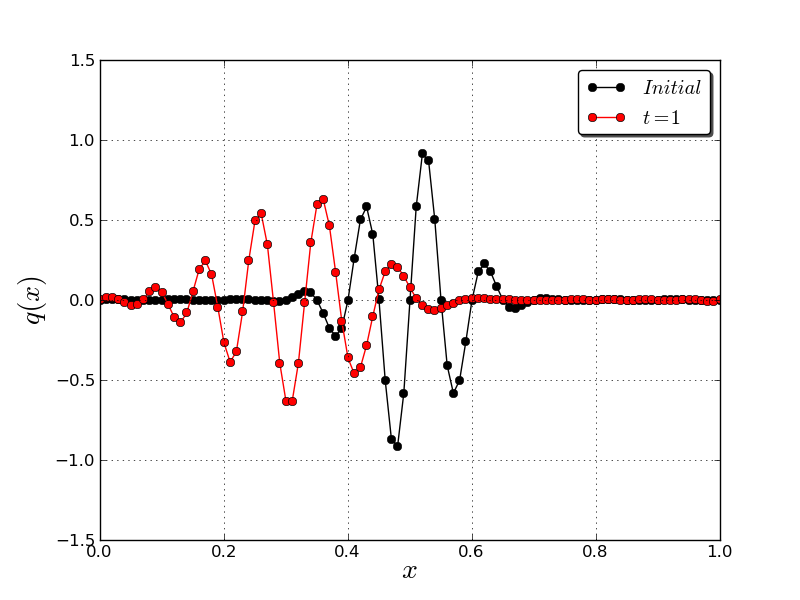
\includegraphics[width=100mm]{Images/wavepacketA.png}
\caption{Convection of wavepacket A with the LW scheme, after 1000 iterations. Black line: Initial solution. Red line: Numerical solution. CFL number is $c=0.1$.}
\label{fig:waveA}
\end{figure}

\noindent {\bf Case B:} Figure~(\ref{fig:waveB}) shows the wavepacket after, supposedly, 0.1 turn ($t=0.1$). It can be seen that the wavepacket has travelled in the opposite direction and is centred around $x=0.4$. Its propagation velocity has thus been around -1. Again, this value is predicted by theory, as Eq.~(\ref{eq:vgroup_LW}) gives the group velocity: $\mathcal{V}_g^{\star} (\pi) \approx -1$ (with a CFL number of 0.1).  

\begin{figure}[h!]
\centering
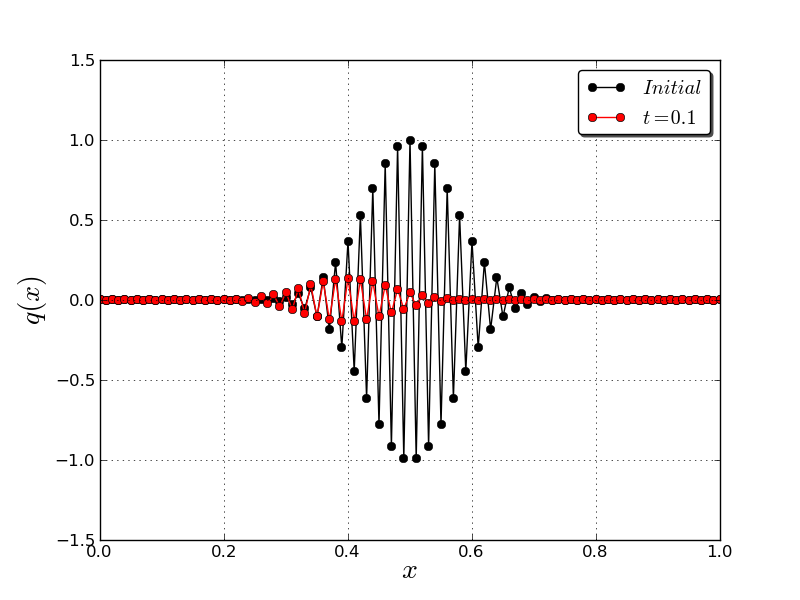
\includegraphics[width=100mm]{Images/wavepacketB.png}
\caption{Convection of wavepacket B with the LW scheme, after 100 iterations. Black line: Initial solution. Red line: Numerical solution. CFL number is $c=0.1$.}
\label{fig:waveB}
\end{figure}

\noindent {\bf Case C:} Figure~(\ref{fig:diffC}) shows the sine wave after, supposedly, 10 turns ($t=10$). It can be seen that the wave suffers from amplitude and phase errors, but in the present case, we are just interested in the former. The wave amplitude is a bit less than 0.9. From Eq.~(\ref{eq:g_LW}), the amplification factor modulus is $\left| g(\pi / 10) \right| \approx 0.999988 $. Then, after 10000 iterations, the initial wave amplitude is multiplied by 0.888, which corresponds the numerical results. 

\begin{figure}[h!]
\centering
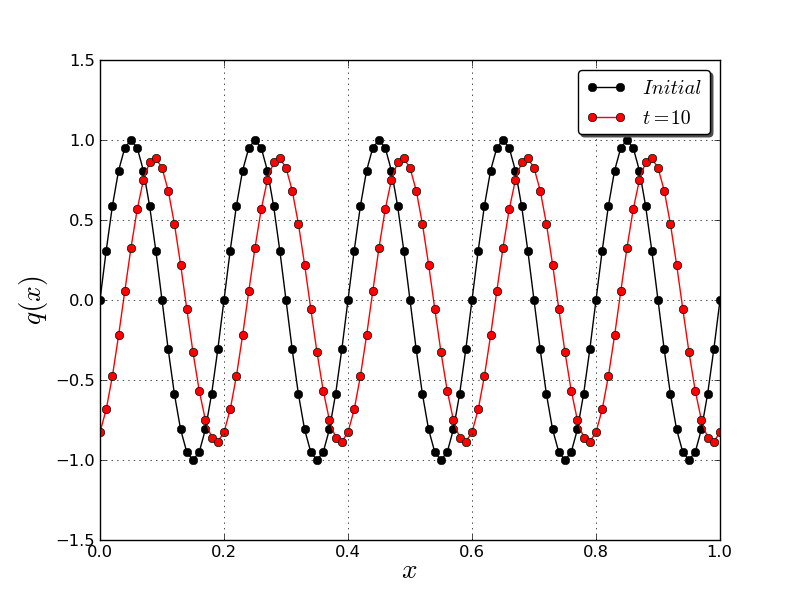
\includegraphics[width=100mm]{Images/diffusion.png}
\caption{Convection of a sine wave with the LW scheme, after 10000 iterations. Black line: Initial solution. Red line: Numerical solution. CFL number is $c=0.1$.}
\label{fig:diffC}
\end{figure}


\noindent This couple of illustrations have shown the interest of spectral analysis in space. It enables to predict the resolution power of a scheme and discriminate physical and spurious waves, depending on phase and group velocities. Moreover, the amount of numerical diffusion introduced by the discretization can also be calculated and $L^2$ stability parameters can be determined. Knowing those main characteristics allows to anticipate many errors when using a numerical scheme. Furtherfore, stabilization or filter operators can be designed to destroy those spurious waves, as it can be seen that their behaviour is non-physical, and often dangerous. 
%--------------


%--------------
% sub 5.2
\subsection{Time analysis}
Similarly to the work of \cite{Trefethen:1982}, we introduce a source term at $x=0.5$ to illustrate the use of time Fourier transforms. We study two kind of source terms:
\begin{itemize}
 \item {\bf Smooth source term D:} The domain is composed with $N_x=200$ knots, the CFL is still $c=0.1$. The source term is defined such that $u(0.5,t)=\sin \left(20 \pi t\right)$, which is $\omega k / c = \pi /10$. After 200 iterations ($t=0.1$), we are supposed to obtain one period of a sine wave, which front has reached $x=0.6$.
 \item {\bf Saw-tooth source term E:} The domain is composed with $N_x=1000$ nodes and is still periodic but also bigger: $\Omega=(0,4)$. The CFL is still $c=0.1$. The source term is such that $u(2,t)=(-1)^n$, then $\omega k / c = 10 \pi $. Thus, it is far greater than the cut-off pulsation. The result is given after 2500 iterations ($t=1$).
\end{itemize}

\noindent {\bf Case D:} Figure~(\ref{fig:sourceD}) shows the results obtained after 200 iterations, which is one period in time for the source term. It can be seen that there is one period of a smooth sine wave at $x>0.5$, which has travelled at $\mathcal{V}_g^{\star} \approx 1$, as expected by theory. On the other hand, there is also some spurious oscillations at $x<0$, which carrier wavelength is around $2 h$. They have travelled at $\mathcal{V}_g^{\star} \approx -1$, as predicted by theory (see Figs.~(\ref{fig:lw_omega}), (\ref{fig:lw_lambdastar_omega}) and (\ref{fig:lw_vgtime})). One should note that the {\it q-waves} are also strongly dissipated, as it can been shown on Fig.~(\ref{fig:mod_lw}).

\begin{figure}[h!]
\centering
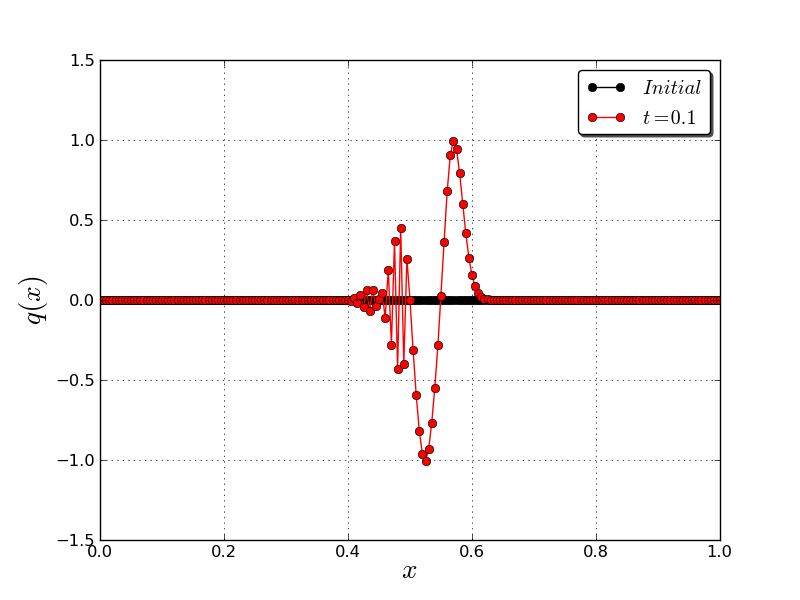
\includegraphics[width=100mm]{Images/sourceD.png}
\caption{Source term D at $x=0.5$. Result after 200 iterations. Black line: Initial solution. Red line: Numerical solution. The scheme is LW and the CFL number is $c=0.1$.}
\label{fig:sourceD}
\end{figure}

\noindent {\bf Case E:} Figure~(\ref{fig:sourceE}) shows the results obtained after 2500 iterations. Voluntarily, the pulsation was chosen far greater than the cut-off pulsation. As theory predicted, nothing can be seen (evanescent waves), except a transient phenomena (see the oscillations for $x \in (2.5,3)$) and the source term itself at $x=2$. If a zoom is made near the source terms, very small and strongly damped oscillations can be seen each side of the source term, with wavelengths close to $4 h$.

\begin{figure}[h!]
\centering
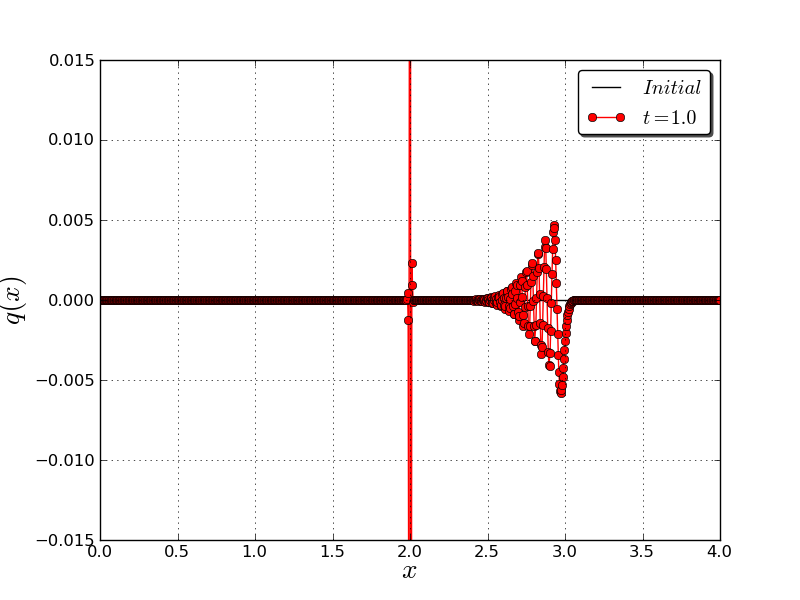
\includegraphics[width=100mm]{Images/sourceE.png}
\caption{Source term E at $x=2$. Result after 2500 iterations. Black line: Initial solution. Red line: Numerical solution. The scheme is LW and the CFL number is $c=0.1$.}
\label{fig:sourceE}
\end{figure}

\noindent Those examples have confirmed the interest of spectral analysis in time. It is probably not to be used as often as space analysis, but the information provided is very precious. Mesh refinement, numerical boundary schemes or the effect of source terms can be studied with this tool. It is thus a good counterpart of space analysis. Moreover, it has the benefit to clearly introduce the notion of characteristic roots and the possible existence of several waves for a given pulsation. 
%--------------


%--------------------------------------------------------------------------------------------------


%--------------------------------------------------------------------------------------------------
% Section n - Conclusion
%==============================
\section{Conclusion \label{sec:conclusion}}
%==============================
This document has presented both space and time spectral analyses to study numerical methods in the frame of the convection-dominated phenomena. As in the works of Vichnevetsky \cite{Vichnevetsky:1982} and Trefethen \cite{Trefethen:1982}, wave propagation definitions, such as the dispersion relation and the group velocity, are introduced and are essential properties to assess a difference scheme. Space analysis is quite classical, as it is closely linked the Von Neumann analysis. The numerical examples given in section~\ref{sec:num_xp} have shown its benefits, especially the use of group velocity to predict the propagation of a wavepacket. 

\noindent On the other hand, time analysis, introduced by Vichnevetsky and Bowles \cite{Vichnevetsky:1982}, is rare and essential yet. Indeed, when the space Fourier transform cannot be used, it is an available and powerful tool. As an example, it enables to determine the group velocities of numerical boundary schemes and thus the spurious reflections at the boundaries \cite{Vichnevetsky:1982}. Another strong argument for time analysis is that Trefethen \cite{Trefethen:1982} has shown the close link between this work due to Vichnevetsky and Bowles \cite{Vichnevetsky:1982} (which gives a physical point of view) and the powerful but complicated \emph{G-K-S (Gustafsson-Kreiss-Sundstr\"om) theory} \cite{GKs:1972} (which is mathematically sound).

\noindent Any linear numerical scheme should be first evaluated with, at least, one of these two tools, before being used to solve more complicated problems (several dimensions, non-linear systems...). In no way, spectral analyses will give fully \emph{sufficient} information about stability or errors for those difficult problems. Nevertheless, having good spectral qualities and robustness when solving Eq.~(\ref{eq:conv_lin}) remains a \emph{ necessity}, if the scheme is used to solve accurately, for instance, the convective terms of the Navier-Stokes equations.

\noindent Those tools will allow to assess the performances of other schemes, like the Taylor-Galerkin family, in a document to come, and then generalized to realize multi-dimensional domains.

%--------------------------------------------------------------------------------------------------

%--------------------------------------------------------------------------------------------------
% Section n+1 - Annexes
%==============================
\appendix
\section{Document Revision History \label{app:revision}}
%==============================

This appendix summarises the main revisions of the present report.

\begin{table}[h]
    \centering
    \label{tab:revision-history}
    \begin{tabular}{p{2cm}p{2.5cm}p{8cm}}
        \toprule
        \textbf{Version} & \textbf{Date} & \textbf{Comment} \\
        \midrule
        1.0 & 2011-01 & Initial report \\
        1.1 & 2026-08 & Few corrections \\
        \bottomrule
    \end{tabular}
	\caption{Document revision history}
\end{table}

%--------------------------------------------------------------------------------------------------

\newpage
\bibliography{NLbiblio}
\bibliographystyle{elsarticle-harv}

%-----------------------------------------------------------
\end{document}
%-----------------------------------------------------------

%===================================================================
